\documentclass{beamer}

\usepackage[pantone3282,english]{wwustyle}

\usepackage[ngerman]{babel}
\usepackage[utf8]{inputenc}
\usepackage[T1]{fontenc}
\usepackage{listings}

\usepackage{graphicx}

% Uncomment the following two lines if you want to prepare your document for
% the fast mode.
% \usetikzlibrary{external}
% \tikzexternalize

\author{Christof, Marius, Thomas}
\title{Multiple RTUs}
%\institutelogo{Logo on title frame}
%\institutelogosmall{Logo on other frames}
\subtitle{Sprint 5}

\begin{document}

%%%%%%%%%%%%%%% WWUstyle "fast" mode %%%%%%%%%%%%%%%%%%%%%
% Do the following steps in order to speed up the compilation time of your
% presentation:
%
% 1. Include the externalization tikz library in the preamble of your document.
%    This is always recommended if you are using tikz in your document.
% 2. Uncomment the \wwupreparefastmode command below
% 3. Compile your document with command line option '-shell-escape',
%    e.g.: 'pdflatex -shell-escape beamer.tex'
% 4. Comment (or delete) the \wwupreparefastmode
% 5. Add option 'fast' to the 'wwustyle' package declaration line.
% 6. Be happy!

% \wwupreparefastmode


\begin{frame}[plain]
	\maketitle
\end{frame}

\begin{frame}
	\frametitle{Inhaltsverzeichnis}
	\begin{itemize}
		\item Topologien
		\item Angriffsszenarien
		\item RTU-Logik
		\item Evaluationsdaten
		\item Operator Tools
		\item Topology Loader
		\item Reflexion
		\item Ausblick
	\end{itemize}
\end{frame}

\begin{frame}
	\frametitle{Topologien}
	\centering
	Topologie 1 und 2
	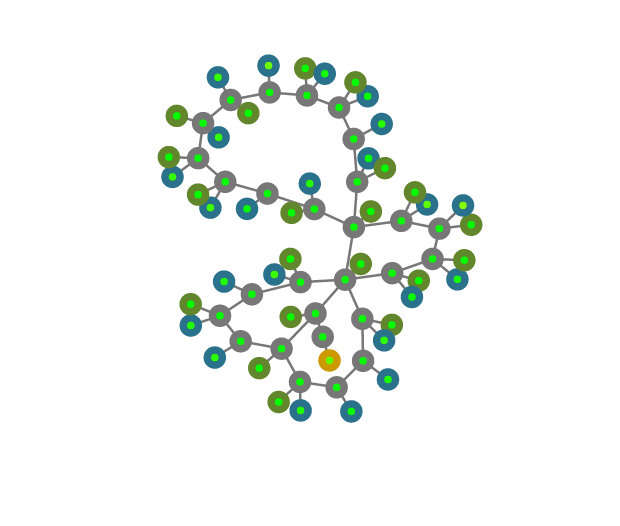
\includegraphics[height=\textheight]{pics/topo_1_2.png}
\end{frame}

\begin{frame}
	\frametitle{Topologien}
	\centering
	Topologie 3 \\
	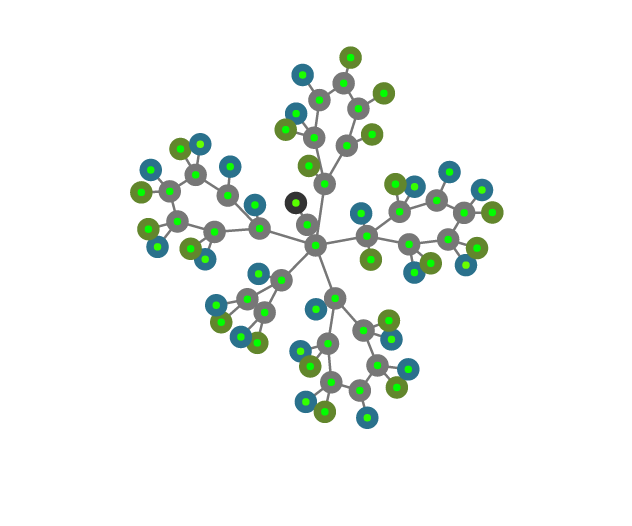
\includegraphics[height=\textheight]{pics/topo_3.png}
\end{frame}

\begin{frame}
	\frametitle{Topologien}
	\centering
	Topologie 4 und 4a
	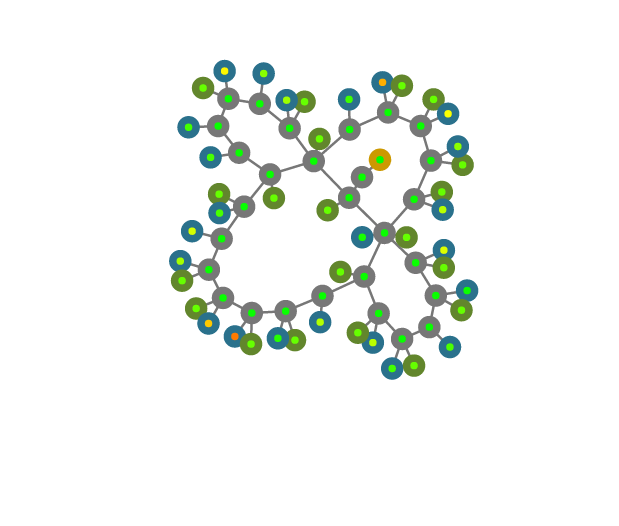
\includegraphics[height=\textheight]{pics/topo_4_4a.png}
\end{frame}

\begin{frame}
	\frametitle{Topologien}
	\centering
	Topologie 5
	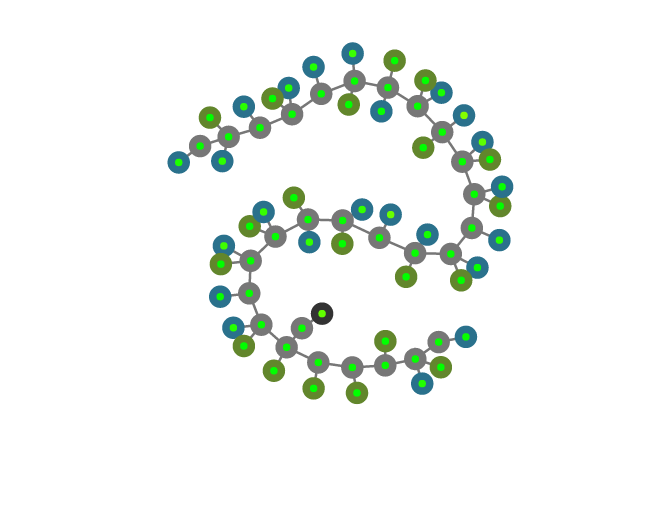
\includegraphics[height=\textheight]{pics/topo_5.png}
\end{frame}

\begin{frame}
	\frametitle{Topologien}
	\centering
	Topologie 6
	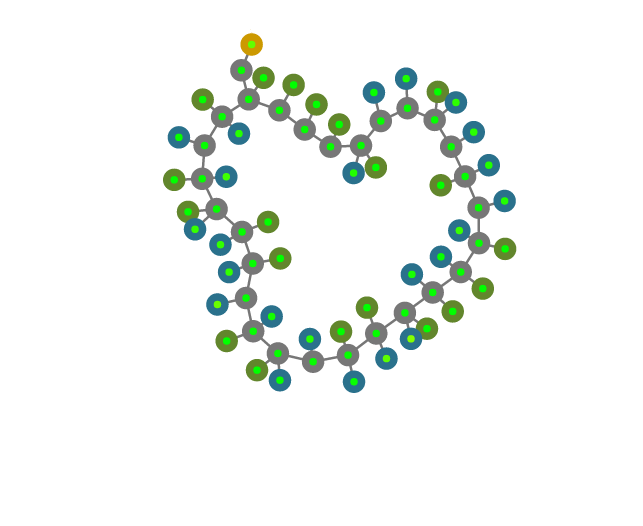
\includegraphics[height=\textheight]{pics/topo_6.png}
\end{frame}

\begin{frame}
	\frametitle{Angriffsszenarien}
	\begin{itemize}
		\item feste Angriffe
		\item randomisierte Angriffe
		\item auf Kirchhoffs Law angepasster Angriff
	\end{itemize}
\end{frame}

\begin{frame}
	\frametitle{RTU-Logik}
	\begin{itemize}
		\item timing Probleme: Logik <> Simulation
		\item Kirchhoffs Law \& R1 haben warning-value
		\item Fix für Kirchhoffs Law ist fehlgeschlagen
		\item trust reset
		\item broadcast bei Angriffserkennung
		\item unsafe Nodes werden nicht überprüft
		\item Mehrheitsentscheidung bei Sensoren an Nodes
	\end{itemize}
\end{frame}

\begin{frame}
	\frametitle{Evaluationsdaten}
	\begin{itemize}
		\item Daten der Simulation können gesammelt werden
		\item Ausgabe als .txt
		\item Visualisierung als Graph
	\end{itemize}
\end{frame}

\begin{frame}
	\frametitle{Operator Tools}
	\begin{itemize}
		\item GUI für den Operator
		\item zeigt Angriffswarnungen der RTUs
		\item gibt Kommando für hard reset
	\end{itemize}
\end{frame}

\begin{frame}
	\frametitle{Topology Loader}
	\begin{itemize}
		\item lädt alle verfügbaren Topologien
		\item schreibt config-Datei für die Simulation
	\end{itemize}
\end{frame}

\begin{frame}
	\frametitle{Reflexion}
	\begin{itemize}
		\item keine Sonderbehandlung der Sensoren am ersten Node nach dem RefBus
		\item Kommandos werden einfach blockiert, nicht angemessen behandelt
		\item current von PVs und Housholds kann nicht für angrenzende RTUs verwendet werden (Kirchhoffs Law)
		\item wenn bei einem als unsafe markiertem Node wirklich ein Fehler auftritt, wird dieser nicht behandelt
	\end{itemize}
\end{frame}

\begin{frame}
	\frametitle{Reflexion}
	\begin{itemize}
		\item Hacker Script Interpreter wirft bei falscher Semantik keine Fehler (sehr zeitaufwändig)
		\item HSI kann leider noch nicht mit floats umgehen
	\end{itemize}
\end{frame}

\begin{frame}
	\frametitle{Ausblick}
	\begin{itemize}
		\item GUI mit Topologie-Loader als Startscreen
		\item RTU Kommunikation erweitern
		\item P3 implementieren
		\item PV/Houshold csv durch Berechnung austauschen
	\end{itemize}
\end{frame}

\begin{frame}
	\centering
	Danke für Ihre Aufmerksamkeit! \\
	Noch Fragen?
\end{frame}

\end{document}
